%version of 02-28-20

\chapter{The hidden beauty of numbers}
\label{Appendix:Tetra}

Our objective here is to develop the reasoning which leads to a proof...

\section{Revisiting triangular numbers}

The $n$ triangular number is equal to the sum of the $n$th first integers.
It is denoted by $\Delta_n$.

$\Delta_n =  \sum_{k=1}^{n} k$

We proved in chapter~\ref{ch:Summation} the expression of $\Delta_n$ by two methods.
\begin{itemize}
\item the trick of Gauss that evidences an invariant (the sum of the $k$th term plus the $n-k+1$th one
is equal to $n+1$. 
\item using the Fubini's double counting principle, the $k$th term is represented by $k$ tokens.
Putting two collections of tokens organized as triangles leads to a rectangle whose surface is equal to $n.(n+1)$.
\end{itemize}
We present below a figure that is an intermediate between both methods and that will serve as the basic principle for further investigations.
Like for Gauss' trick, the sum of each row is an invariant (see the last column of Fig.~\ref{fig:Tetrahedral2}). 

\begin{figure}[h]
\begin{center}
        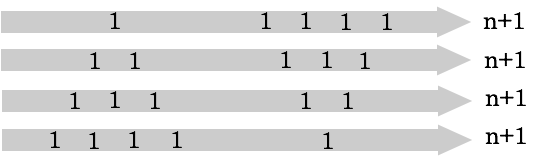
\includegraphics[scale=0.4]{FiguresArithmetic/appTetrahedral2}
        \caption{Computing $\Delta_n$: two copies of a basic triangle pattern.}
        \label{fig:Tetrahedral2}
\end{center}
\end{figure}
$\Delta_n =  \sum_{k=1}^{n} k = \frac{1}{2}n.(n+1)$


\section{Tetrahedral numbers}
\label{sec:tetraedralNumbers}

The problem here is to compute:

$\Theta_n =  \sum_{k=1}^{n} \Delta_k$


\subsection{A first look}

The natural way is to replace $\Delta_k$ by its value $\frac{n.(n+1)}{2}$ and to determine the expression
by arithmetic manipulations.

We left this task to the readers, the expression is:

$\Theta_n =  \sum_{k=1}^{n} \Delta_k $

$=  \sum_{k=1}^{n} \frac{1}{2} (k^2 + k) $

$=  \frac{1}{2} (\sum_{k=1}^{n} k^2 + \sum_{k=1}^{n} k) $

Using expression~\ref{eq:sum-1-to-nsq} for the sum of squares:

$= \frac{1}{2} ( \frac{1}{3} n^3 + \frac{1}{2} n^2 + \frac{1}{6} n + \frac{1}{2} n^2 + \frac{1}{2} n )$

$= \frac{n.(n+1).(n+2)}{6}$

\medskip

Remark that this result can also easily been proved by recurrence as soon as the expression is known
(by guessing the expression).
We let the reader develop this proof. 


\subsection{A pictorial proof}

We suggest to use the double counting Fubini's principle.

Following this way, you should write the previous expression of the tetrahedral number in a developed form 
using a triangle shape as shown in Fig.~\ref{fig:Tetrahedral2}.

draw two copies by rotating the dimensions.

Fubini's principle is used by summing up the successive rows.

Prove as an intermediate result that the sum of the elements over the rows of the three triangles is proportional to $n+2$.
\medskip

\noindent \fbox{
\begin{minipage}{0.96\textwidth}
{\bf Explanatory note}.

to be completed
\end{minipage}
}
\medskip

We will extend the previous construction to prove the expression of $\Theta_n$.
The idea is to consider three copies and organize them in order to obtain the expected result.

A tetrahedral number is the sum of triangular numbers, and thus, it can be arranged as a triangle (see Fig.~\ref{fig:Tetrahedral3}).
%\begin{figure}[h]
%\begin{center}
%        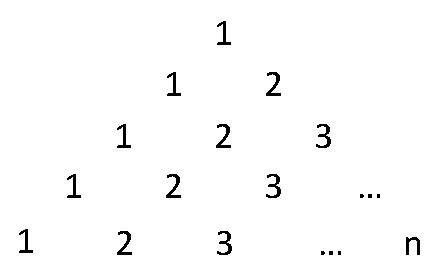
\includegraphics[scale=0.5]{FiguresArithmetic/TetrahedralBasic}
%        \caption{Computing $\Theta_n$: basic triangle pattern.}
%        \label{fig:TetrahedralBasic}
%\end{center}
%\end{figure}

The proof is obtained by the double counting principle by rotating the three faces of triangles as shown in Fig.~\ref{fig:Tetrahedral1}.
\begin{figure}[h]
\begin{center}
        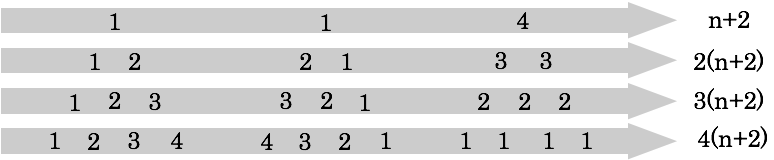
\includegraphics[scale=0.4]{FiguresArithmetic/appTetrahedral3}
        \caption{Basic pattern for computing $\Theta_n$ (for $n=4$).}
        \label{fig:Tetrahedral3}
\end{center}
\end{figure}
\begin{figure}[h]
\begin{center}
        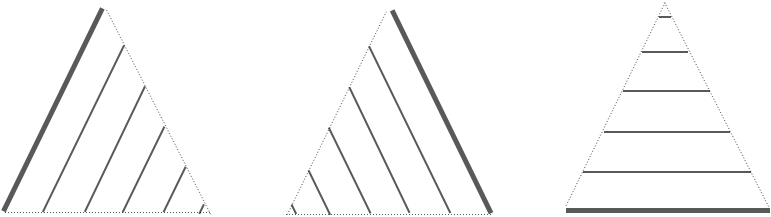
\includegraphics[scale=0.3]{FiguresArithmetic/appTetrahedral1}
        \caption{Computing $\Delta_n$: basic triangle pattern.}
        \label{fig:Tetrahedral1}
\end{center}
\end{figure}

Sum up all the numbers in each row.

\begin{itemize}
\item 
The first row is equal to $1+1+n = n+2$.
\item
The second one is equal to $3 + 3 + 2(n-1) = 2(n+2)$. 
\item
Let us sum up the elements in row $k$: 

$\Delta_k + \Delta_k + k(n-k+1)  = k(k+1) + kn-k^2+k = k(n+2)$.
\end{itemize}


$= \frac{1}{4}.\Theta_n.(n+3)$
\begin{figure}[h]
\begin{center}
        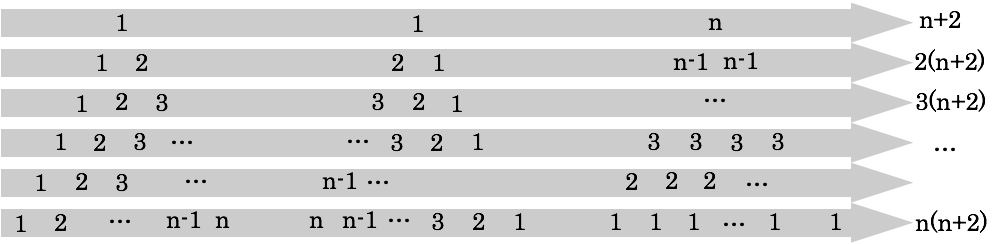
\includegraphics[scale=0.32]{FiguresArithmetic/appTetrahedral4}
        \caption{Computing $\Theta_n$: basic triangle pattern.}
        \label{fig:Tetrahedral4}
\end{center}
\end{figure}
The global sum is equal to $n+2$ times $(1+2+...+n)$.

Finally, $3 \Theta_n = (n+2) \Delta_n$
\medskip

\noindent \textit{Summary:} we proved the following results:
\begin{itemize}
\item $Id_n = 1+1+ ... +1 = n$
\item $\Delta_n = 1+2+3+ ... +n = \frac{1}{2}.Id_n.(n+1) = = \frac{n.(n+1)}{2}$
\item $\Theta_n = \Delta_1 + \Delta_2 + ... + \Delta_n = \frac{1}{3} .\Delta_n.(n+2) = \frac{1}{3}.\Delta_n.(n+2) = \frac{n.(n+1).(n+2)}{3!}$
\end{itemize}


\section{$\oplus$ Pentahedral numbers}

As the previous results show some regularities, a natural question is: \textit{can we go further following the same pattern for computing 
$ \sum_{k=1}^{n} \Theta_k$?}

Looking at the successive expressions, the expectation is ...

$\Pi_n = \Theta_1 + \Theta_2 + ... + \Theta_n = \frac{1}{4}.\Theta_n.(n+3) = \frac{n.(n+1).(n+2).(n+3)}{4!} $

\begin{figure}[h]
\begin{center}
        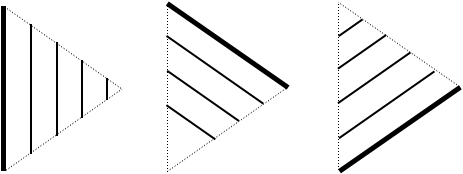
\includegraphics[scale=0.35]{FiguresArithmetic/appTetrahedral6}
        \caption{Computing $\Pi_n$: basic triangle pattern.}
        \label{fig:Tetrahedral6}
\end{center}
\end{figure}
\begin{figure}[h]
\begin{center}
        \includegraphics[scale=0.36]{FiguresArithmetic/appTetrahedral7}
        \caption{Computing $\Pi_n$: basic triangle pattern (for $n=4$).}
        \label{fig:Tetrahedral7}
\end{center}
\end{figure}

Finally

\begin{figure}[h]
\begin{center}
        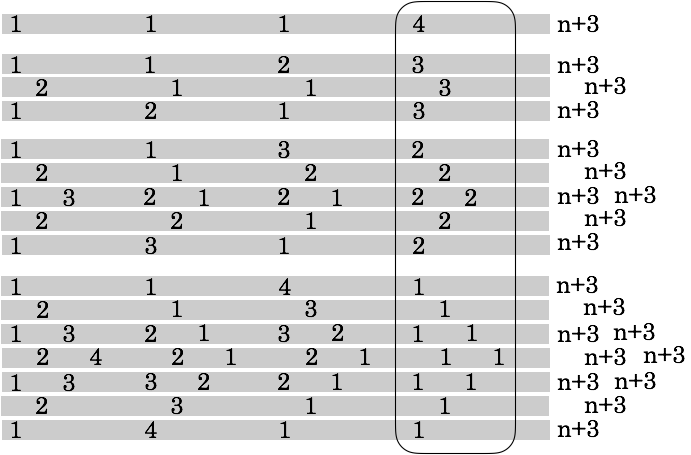
\includegraphics[scale=0.36]{FiguresArithmetic/appTetrahedral5}
        \caption{Add the last first $\Theta_n$ and sum up the rows and then, the last columns.}
        \label{fig:Tetrahedral5}
\end{center}
\end{figure}


\subsection{Going further}

Are you able to consider the challenge of going one step further?

We expect the sum of pentahedral numbers to be equal to:

$\frac{1}{5}.\Pi_n.(n+4) = \frac{n.(n+1).(n+2).(n+3).(n+4)}{5!}$




